%----------------------------------------------------------------------------------------
%  PACKAGES AND CONFIGURATION
%----------------------------------------------------------------------------------------

\documentclass{rapport}
\usepackage{geometry}
\usepackage{fancyhdr} % For custom headers
\usepackage{lastpage} % To determine the last page for the footer
\usepackage{float}
\usepackage{extramarks} % For headers and footers
\usepackage[most]{tcolorbox} % For problem answer sections
\usepackage{graphicx} % For inserting images
\usepackage{xcolor} % For link coloring
\usepackage[hidelinks]{hyperref} % For URL links (no box or color name) 

%Ce que moi(Alban) ai rajouté comme package
\usepackage{comment} 
\usepackage{multicol} % Pour les colonnes
\usepackage{listings}
\usepackage{courier}
\usepackage{subcaption}

\definecolor{backcolour}{RGB}{47,47,47}
\definecolor{violet}{RGB}{200,20,200}
\definecolor{codegreen}{rgb}{0,0.6,0}
\definecolor{codegray}{rgb}{0.5,0.5,0.5}
\definecolor{marron}{RGB}{150,100,70}
\definecolor{red2}{RGB}{207,43,58}
\definecolor{bordeaux}{RGB}{74,31,30}
\lstdefinestyle{mystyle}{
    language=Python,
    basicstyle=\tiny\ttfamily
    backgroundcolor=\color{backcolour},   
    commentstyle=\color{codegreen},
    keywordstyle=\color{violet},
    numberstyle=\tiny\color{codegray},
    stringstyle=\color{red},
    literate={,}{{\textcolor{red}{,}}}1
             {;}{{\textcolor{red}{;}}}1,
    basicstyle=\ttfamily\footnotesize,
    breakatwhitespace=false,         
    breaklines=true,                 
    captionpos=b,                    
    keepspaces=true,                 
    numbers=left,                    
    numbersep=5pt,                  
    showspaces=false,                
    showstringspaces=false,
    showtabs=false,                  
    tabsize=2,
    literate=
  {á}{{\'a}}1 {é}{{\'e}}1 {í}{{\'i}}1 {ó}{{\'o}}1 {ú}{{\'u}}1
  {Á}{{\'A}}1 {É}{{\'E}}1 {Í}{{\'I}}1 {Ó}{{\'O}}1 {Ú}{{\'U}}1
  {à}{{\`a}}1 {è}{{\`e}}1 {ì}{{\`i}}1 {ò}{{\`o}}1 {ù}{{\`u}}1
  {À}{{\`A}}1 {È}{{\'E}}1 {Ì}{{\`I}}1 {Ò}{{\`O}}1 {Ù}{{\`U}}1
  {ä}{{\"a}}1 {ë}{{\"e}}1 {ï}{{\"i}}1 {ö}{{\"o}}1 {ü}{{\"u}}1
  {Ä}{{\"A}}1 {Ë}{{\"E}}1 {Ï}{{\"I}}1 {Ö}{{\"O}}1 {Ü}{{\"U}}1
  {â}{{\^a}}1 {ê}{{\^e}}1 {î}{{\^i}}1 {ô}{{\^o}}1 {û}{{\^u}}1
  {Â}{{\^A}}1 {Ê}{{\^E}}1 {Î}{{\^I}}1 {Ô}{{\^O}}1 {Û}{{\^U}}1
  {œ}{{\oe}}1 {Œ}{{\OE}}1 {æ}{{\ae}}1 {Æ}{{\AE}}1 {ß}{{\ss}}1
  {ű}{{\H{u}}}1 {Ű}{{\H{U}}}1 {ő}{{\H{o}}}1 {Ő}{{\H{O}}}1
  {ç}{{\c c}}1 {Ç}{{\c C}}1 {ø}{{\o}}1 {å}{{\r a}}1 {Å}{{\r A}}1
  {€}{{\EUR}}1 {£}{{\pounds}}1
}

\title{TS229}
\begin{document}

%----------- Informations du rapport ---------
\logo{images/logo_em.jpg}
\unif{École nationale supérieure d'électronique, informatique, télécommunications, mathématiques et mécanique de Bordeaux}
\titre{Lecture de code-barres par lancers aléatoires de rayons}
\cours{Département Télécom} %Nom du cours
\sujet{TS225 : Projet Images} %Nom du sujet
\enseignant{Marc \textsc{DONIAS}}
\eleves{Elisa \textsc{Chien} \\
		Alban \textsc{Oberti} \\
		Tierno-Alpha \textsc{Tall} \\
		David \textsc{Yan} 
		}

%----------------------------------------------------------------------------------------
%   TITLE PAGE
%----------------------------------------------------------------------------------------
\fairemarges %Afficher les marges
\fairepagedegarde %Créer la page de garde
\newpage
\tabledematieres %Créer la table de matières
\newpage
% ------------------------------------------------ %

\section{Introduction}

\section{Algorithmes}

\subsection{Phase 1 : Détection du code barre}
\subsection{Phase 2 : Lecture du code barre}

La phase précédente a permis de récupérer un ensemble de couple de points représentant des rayons. 
Pour chaque couple de points, nous déterminons d'une part les 13 valeurs du code barre, et d'autre part, s'il est valide ou non.

\subsubsection*{Seuillage à l'aide d'Otsu}
La méthode d'Otsu est une technique de seuillage utilisée en traitement d'images pour la segmentation binaire. 
Elle vise à séparer les pixels d'une image en deux classes distinctes : l'avant-plan et l'arrière-plan. 
L'algorithme d'Otsu fonctionne en cherchant le seuil de gris qui minimise la variance intra-classe, c'est-à-dire la somme des variances des deux classes. 
Pour ce faire, il calcule l'histogramme des niveaux de gris de l'image et évalue la dispersion des pixels pour chaque seuil possible. 
Le seuil optimal est celui qui maximise la variance inter-classe, assurant ainsi une séparation claire entre les deux classes. 
En pratique, le seuil calculé devrait se situer entre les deux pics de l'histogramme.

\subsubsection*{Détermination des limites du code-barres}
\subsubsection*{Détermination du dernier chiffre du code barre}

À partir des six premières valeurs obtenues, nous pouvons déterminer le premier chiffre. 
Il suffit ainsi de lire le tableau de correspondance suivant :

\begin{table}[h!]
    \centering
    \renewcommand{\arraystretch}{1.5} % Ajuste l'espacement vertical
    \begin{tabular}{|c|c|c|c|}
        \hline
        \textbf{Séquence} & \textbf{1\textsuperscript{er} Chiffre} & \textbf{Séquence} & \textbf{1\textsuperscript{er} Chiffre} \\ \hline
        AAAAAA & 0 & ABBAAB & 5 \\ \hline
        AABABB & 1 & ABBBAA & 6 \\ \hline
        AABBAB & 2 & ABABAB & 7 \\ \hline
        AABBBA & 3 & ABABBA & 8 \\ \hline
        ABAABB & 4 & ABBABA & 9 \\ \hline
    \end{tabular}
    \caption{Tableau des familles d’appartenance de la première séquence}
    \label{tab:sequence}
\end{table}

\subsubsection*{Analyse du code barre binaire}

\section{Vérification de la clef de contrôle}

\subsection{Phase 1 : Détection du code barre}
\subsection{Phase 2 : Lecture du code barre}

\section{Résultats}

\subsubsection*{Seuillage à l'aide d'Otsu}
Prenons l'image suivante :
\begin{figure}[H] % Ajouter les deux points reçu en argument 
	\centering
	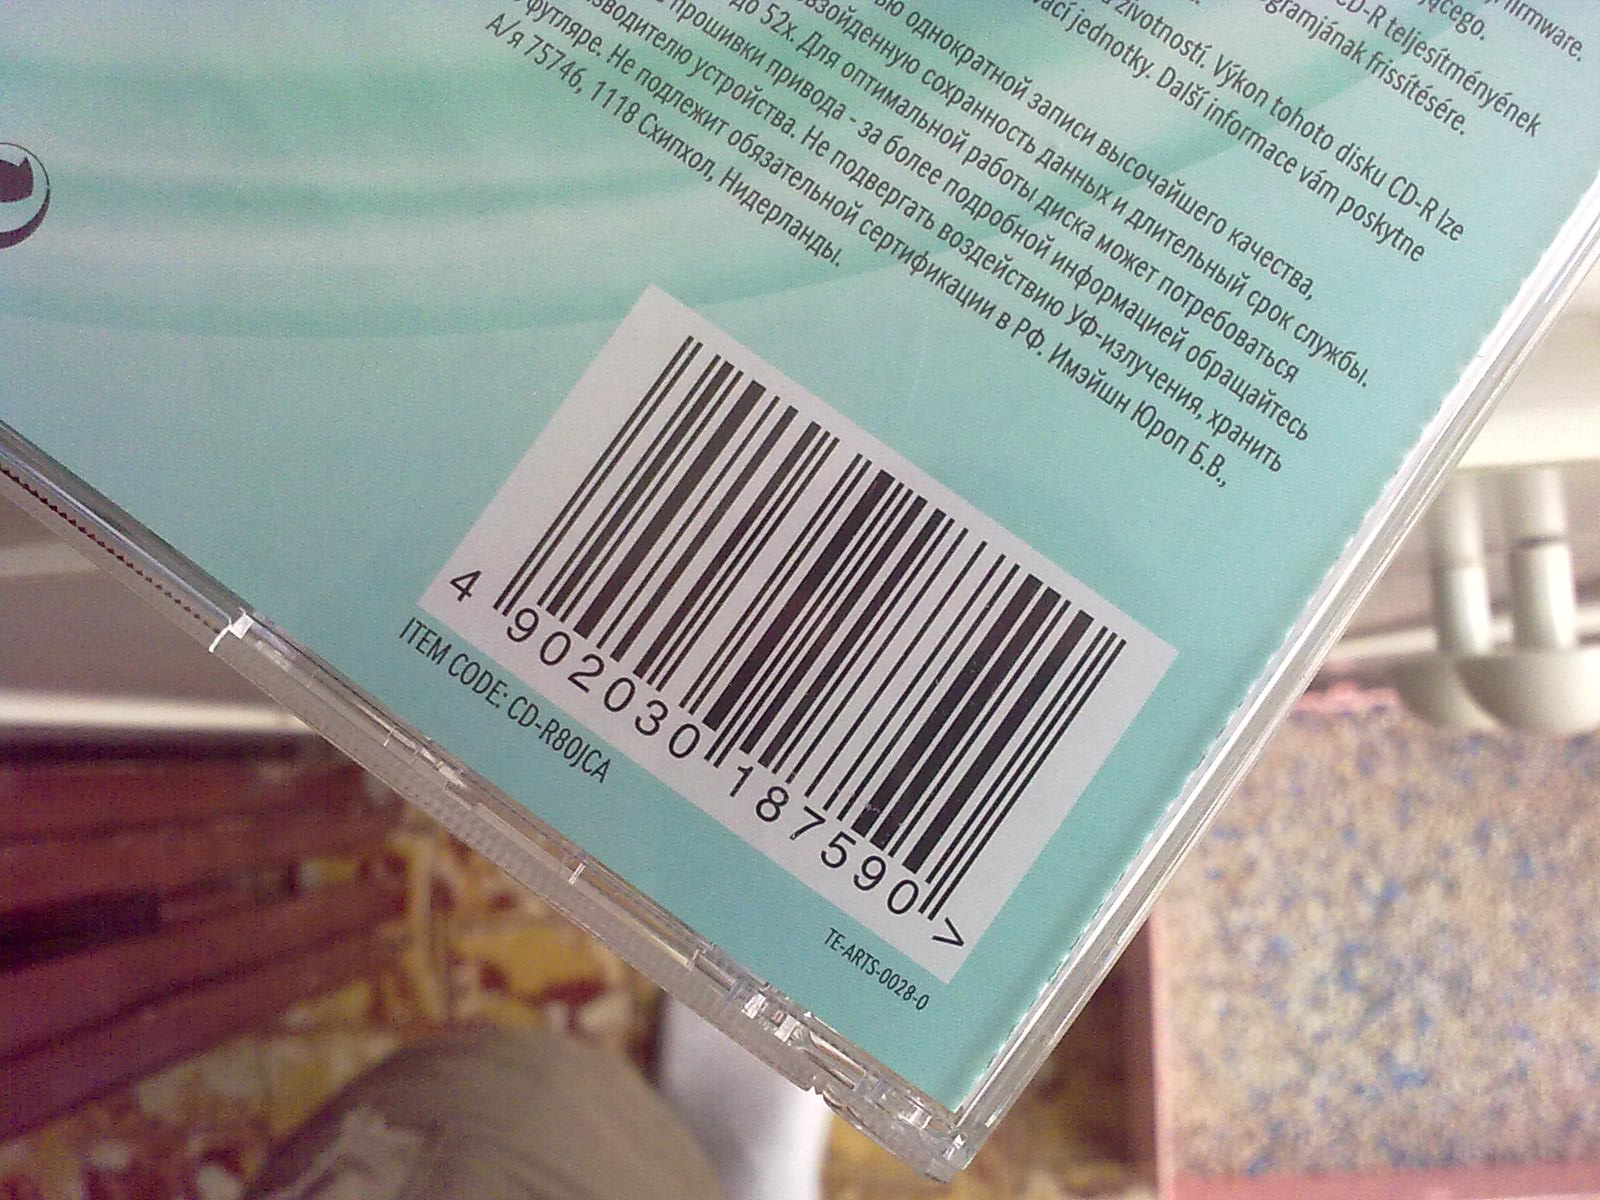
\includegraphics[width=0.5\textwidth]{images/barcode0.jpg}
	\caption{Image d'un code barre}
	\label{code_barre}
\end{figure}

Avant cela de pouvoir lire un code barre, nous devons opérer un seuillage de l'image. Pour cela, nous utilisons la méthode d'Otsu.
Cette méthode repose sur le calcul d'un seuil optimal pour binariser une image en niveaux de gris.
Ce seuil est déterminé grâce à l'histogramme de l'image et est censé séparer les pixels en deux classes distinctes : les pixels noirs et les pixels blancs.

Pour la figure \ref{code_barre}, nous obtenons l'histogramme suivant :

\begin{figure}[H] 
	\centering
	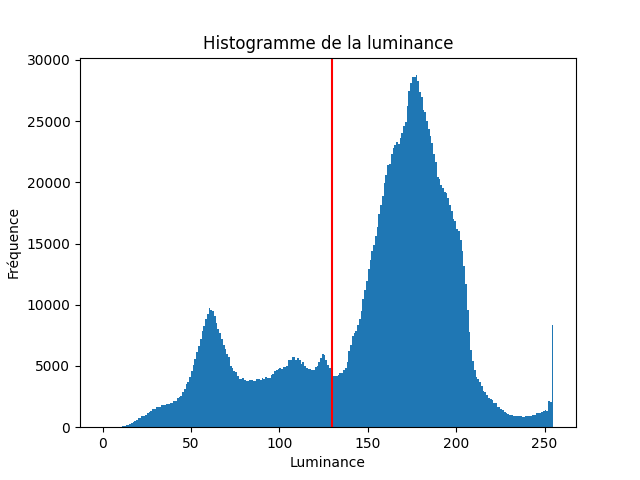
\includegraphics[width=0.5\textwidth]{images/histogramme.png}
	\caption{Histogramme de l'image}
	\label{histogramme}
\end{figure}

Grâce à ce seuil, nous obtenons ainsi l'image seuillée : 
% Ajouter image seuillée avec Otsu

\subsubsection*{Détermination des limites du code-barres}
\subsubsection*{Détermination du dernier chiffre du code barre}
\subsubsection*{Analyse du code barre binaire}






\subsubsection*{Détermination des limites du code-barres}

\subsubsection*{Détermination du dernier chiffre du code barre}

\subsubsection*{Analyse du code barre binaire}

\section{A ENLEVER : Phase 2 : Lecture du code barre}

\subsection{Seuillage de l'image avec Otsu}



\subsection{Détermination des limites du code-barres}

Le rayon initial traverse potentiellement des zones inutiles de l'image. Il est donc essentiel de réduire ce segment pour que ses extrémités coïncident avec les bords du code-barres (les premières barres noires détectées).  
Cette première étape est réalisée en échantillonnant l’image le long du segment défini, puis en appliquant un seuil de binarisation. Ce seuil est calculé grâce à l’algorithme d’Otsu.  

% Afficher l'image avec les deux points reçu en argument
\begin{figure}[H] % Ajouter les deux points reçu en argument 
	\centering
	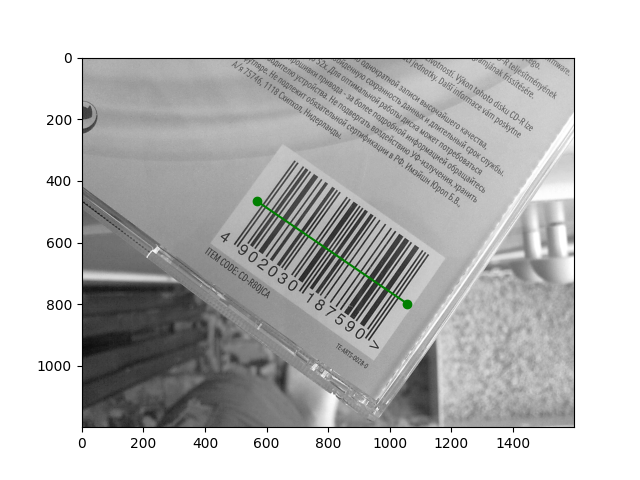
\includegraphics[width=0.5\textwidth]{images/code_barre_couple_vert.png}
	\caption{Segment défini par le deux points en arguments}
\end{figure}

La première étape de cette phase est de réduire ce rayon, de sorte que les deux nouveaux points correspondent à la première barre noire du code barre.
Pour cela, nous devons tout d'abord opérer un seuillage de l'image grâce au seuil donné par l'algorithme d'otsu.
Le segment est alors échantilloné en prenant le plus proches voisins. 
Cet ensemble de points va alors être binarisé grâce au seuil.

\begin{figure}[H] 
	\centering
	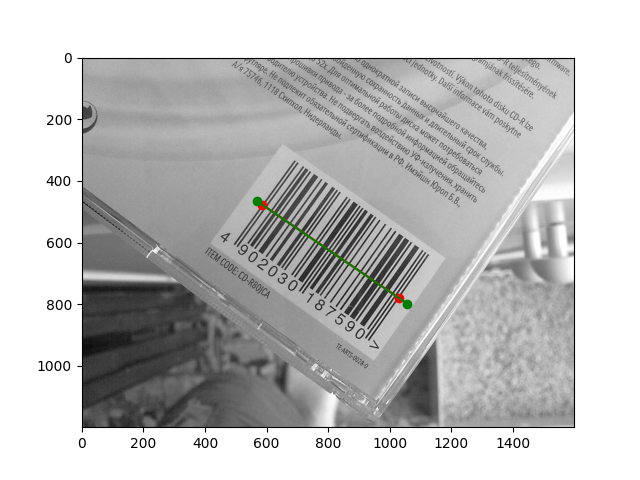
\includegraphics[width=0.5\textwidth]{images/binarisation.png}
	\caption{Délimitation}
	\label{fig:binarisation}
\end{figure}

Les points déterminant le début et la fin du code-barres sont ensuite déterminés en prenant le premier et dernier point de valeur 0

\begin{figure}[H] 
	\centering
	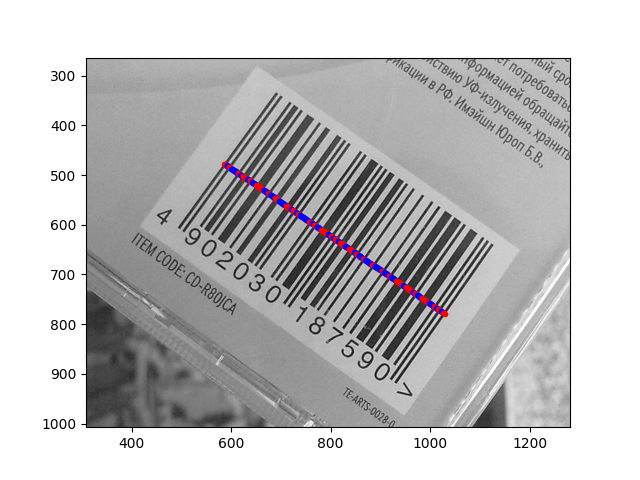
\includegraphics[width=0.5\textwidth]{images/detection.png}
	\caption{Détection du noir et blanc}
	\label{fig:detection}
\end{figure}

Finalement un dernier échantillonnage suivi d'une binarisation sur le même seuil permet de trouver la liste binaire à analyser
Le nombre de point échantillonnés est calculé en prenant $N=u*95$ avec u le plus petit multiple de 95 tel que u*95>L la longueur du segment du code barre

\subsection{Analyse du code barre binaire}
La prochaine étape consiste à séparer les différents blocs contenu dans la liste binaire obtenu précédemment en ne gardant que ceux représentant des nombres
Pour décoder chaque blocs, ils font être comparé avec des données de décodage en adaptant celle-ci à la taille du bloc 
Le choix se fera en prenant la plus petit norme entre le bloc et les données comparés. 

\subsection{Détermination du dernier chiffre du code barre}

\subsection{Vérification de la clef de contrôle}
Nous obtenons finalement pour cette image le code \textbf{4902030187590}, ce qui correspond bien au code barre présent sur l'image.
De manière générale, il faut tout de même vérifier la validité du code barre. Pour cela, nous suivons l'algorithme de vérification de code barre grâce à la clé de contrôle.

En l'occurrence, le complément à 10 du dernier chiffre du code barre vaut 0, tandis que le chiffre des unités de la somme des chiffres de rang impair et trois fois la somme des chiffres de rang pair vaut 0. 
Le code barre est donc valide.

\section{Mise en commun des deux phases}

\section{Bilan de l'organisation}

\subsection{Séance 1}

\begin{table}[htbp]
	\centering 
	\begin{tabular}{c|c|c}
		& Tâches entreprises& Temps passé\\ \hline
		Elisa& Prise de connaissance du sujet et commencement de la méthode d'Otsu& 2h\\ \hline
		Alban& Lecture et analyse du sujet et début de l'implémentation d'algorithme d'échantillonnage et de binarisation& 2h\\ \hline
		Tierno& & \\ \hline
		David& & 
	\end{tabular}
	\caption{Organisation de la séance 1}
\end{table}

\subsection{Séance 2}

\begin{table}[htbp]
	\centering 
	\begin{tabular}{c|c|c}
		& Tâches entreprises& Temps passé\\ \hline
		Elisa& Finition de la méthode d'Otsu & 2h\\ \hline
		Alban& Complétion de l'échantillonnage et de la binarisation, début du calcul des limites du code-barres et de la recherche de u& 2h\\ \hline
		Tierno& & \\ \hline
		David& & 
	\end{tabular}
	\caption{Organisation de la séance 2}
\end{table}

\subsection{Séance 3}

\begin{table}[htbp]
	\centering 
	\begin{tabular}{c|c|c}
		& Tâches entreprises& Temps passé\\ \hline
		Elisa& Débuggage et mise en commun de toutes les fonctions de la phase 1 & 3h\\ \hline
		Alban& Débuggage des fonctions de décodage des blocs fait chez soi et mise en commun du travail phase1& 3h\\ \hline
		Tierno& & \\ \hline
		David& & 
	\end{tabular}
	\caption{Organisation de la séance 3}
\end{table}

\subsection{Séance 4}

\begin{table}[htbp]
	\centering 
	\begin{tabular}{c|c|c}
		& Tâches entreprises& Temps passé\\ \hline
		Elisa& & \\ \hline
		Alban& Dernier débuggage et test sur des exemples pour vérifier l'efficacité du code& 3h\\ \hline
		Tierno& & \\ \hline
		David& & 
	\end{tabular}
	\caption{Organisation de la séance 4}
\end{table}

\subsection{Séance 5} % 13 Décembre 

\newpage

\section{Annexes}

\lstset{style=mystyle}

\subsection{Méthode d'Otsu}
\begin{multicols}{2}
	\begin{lstlisting}
		def otsu(img, bins=255, displayHisto=False):
		luminance = None
		
		# Si l'image est en couleur (3 dimensions)
		if len(img.shape) == 3 and img.shape[2] > 1:
			# Calcul de la luminance 
			luminance = np.array([[(img[i][j][0] + img[i][j][1] + img[i][j][2])//3 for j in range(img.shape[1])] for i in range(img.shape[0])])
			luminance = luminance.ravel()
		else:
			luminance = img.ravel()
		
		# Création de l'histogramme
		histogram, bin_edges = np.histogram(luminance.ravel(), range=(0, 255), bins=bins)
		
		# Moyenner l'histogramme
		histogram = histogram/sum(histogram)    
		
		# Création d'un dico pour associer chaque valeur de luminance à sa fréquence
		histogram_dic = {int(bin_edges[i]): histogram[i] for i in range(len(histogram))}
		
		# Initialisation des moyennes et poids initiaux
		n = len(histogram_dic)
		sumB = 0
		wB = 0
		maximum = 0.0
		sum1 = sum(i * histogram_dic[i] for i in range(n))
		total = sum(histogram_dic.values())
		level = 0
		for k in range(1, n):
			wF = total - wB
			if wB > 0 and wF > 0:
				mF = (sum1 - sumB) / wF
				val = wB * wF * (sumB / wB - mF) * (sumB / wB - mF)
				
				if val >= maximum:
					level = k
					maximum = val
			
			wB += histogram_dic[k]
			sumB += (k-1) * histogram_dic[k]
		
		# Afficher l'histogramme
		if displayHisto:
			plt.figure()
			plt.hist(luminance, bins=bins, range=(0, 255))
			plt.axvline(level, color='r')
			plt.title("Histogramme de la luminance")
			plt.xlabel("Luminance")
			plt.ylabel("Fréquence")
			plt.show()
		
		return level
	
	\end{lstlisting}
\end{multicols}

\end{document}